Per lo sviluppo della parte relativa alla GUI è stato adottato il design pattern \textit{Model-View}. \newline
All'avvio dell'applicazione viene visualizzata la finestra principale \texttt{MainWindow} che è derivata pubblicamente da \texttt{QMainWindow}. \newline
\begin{wrapfigure}{l}{0.6\textwidth}
    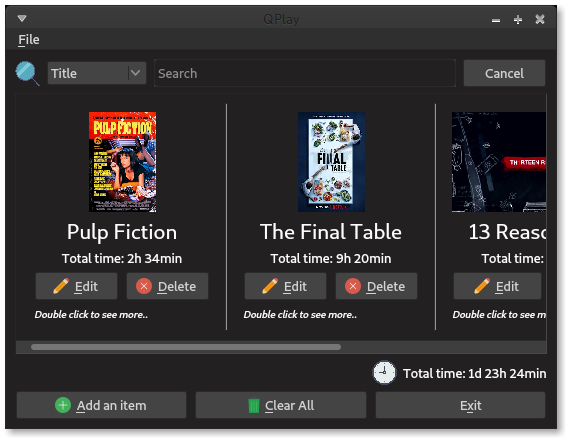
\includegraphics[width=0.6\textwidth]{img/main} 
\end{wrapfigure}
È composta da una \textit{Tool bar} attraverso il quale si può scegliere di caricare una lista di AudioVisual già esistente, salvare la lista corrente oppure uscire dall'applicazione. \newline

Si ha poi a disposizione una barra di ricerca in cui si può cercare in base a diversi filtri, per ognuno dei quali vengono visualizzati i corrispettivi widget di ricerca. La ricerca è stata implementata in modo che sia \textit{case insensitive} e \textit{real time}. \newline
Ogni volta che viene cambiato il filtro di ricerca, la ricerca precedente viene resettata, ritornando così alla lista principale contenente tutti gli elementi della lista. \newline

Nella fascia centrale di \texttt{MainWindow} si trova una lista di \texttt{AudioVisualItem} che derivano pubblicamente da \texttt{QWidget}. Questo widget ha lo scopo di mostrare i dettagli principali di ciascun oggetto contenuto nella lista. \newline
Contiene inoltre due bottoni che servono per richiamare la funzione di modifica e la funzione di eliminazione dell'elemento che rappresentano. \newline
Quando viene cliccato il bottone per la modifica viene mostrata la finestra \texttt{EditWidget}, derivata pubblicamente da \texttt{QWidget}. Esso si occupa di modificare l'elemento della lista selezionato. \newline 
Mentre nella finestra di dialogo per l'aggiunta di un nuovo oggetto si può scegliere il tipo, nella finestra relativa alla modifica non si può modificare il tipo dell'elemento.
%Ogni volta che viene applicato un filtro di ricerca la lista mostra solo i widget che rappresentano i risultati corretti della ricerca. \newline
\begin{wrapfigure}{r}{0.6\textwidth}
    
\includegraphics[width=0.6\textwidth]{img/add} 
\end{wrapfigure}
Quando viene fatto doppio click su un elemento della lista viene aperta la finestra \texttt{DisplayWidget}, derivata pubblicamente da \texttt{QDialog}, con cui vengono visualizzati tutti i dettagli relativi all'oggetto selezionato. \newline

Nella parte più bassa della finestra principale vengono resi disponibili tre bottoni che servono per aggiungere un nuovo elemento alla lista, uno che si occupa di cancellare l'intera lista, uno per uscire dall'appplicazione. \newline 

Quando viene premuto il bottone per l'aggiunta viene aperta una nuova finestra di dialogo denominata \texttt{AddDialog} che deriva pubblicamente da \texttt{QDialog}. \newline
Come prima cosa viene consigliato di scegliere il tipo dell'oggetto che si vuole aggiungere, infatti, in base a quello i widget mostrati nella finestra cambiano permettendo all'utente di inserire i campi dati realtivi ad ogni tipo scelto, che rappresentano le classi concrete della gerarchia. \newline 
